\documentclass[tikz,border=8pt]{standalone}
% Shared look for every TikZ diagram. Load with \input{../../tools/tikz-style.tex}
\usepackage[T1]{fontenc}
\usepackage{lmodern}
\renewcommand{\sfdefault}{lmr}  % diagrams use the same serif as the text
\usetikzlibrary{arrows.meta, positioning, shapes.geometric, calc, fit, backgrounds}
\definecolor{cblue}{HTML}{4C78A8}
\definecolor{corange}{HTML}{F58518}
\definecolor{cgreen}{HTML}{54A24B}
\definecolor{cred}{HTML}{E45756}
\definecolor{cpurple}{HTML}{B279A2}
\definecolor{cgrey}{HTML}{6B6B6B}
\tikzset{
  every picture/.style={font=\sffamily, line width=1.2pt},
  box/.style={draw=#1, fill=#1!12, rounded corners=4pt, align=center, inner sep=7pt, minimum height=1.1cm},
  box/.default=cgrey,
  arrow/.style={-{Stealth[length=3mm]}, draw=cgrey, line width=1.4pt},
  title/.style={font=\sffamily\bfseries\Large},
  note/.style={font=\sffamily\small, text=cgrey, align=center},
}
\AtBeginDocument{\hyphenpenalty=10000 \exhyphenpenalty=10000}

\begin{document}
\begin{tikzpicture}[
  inp/.style={circle, draw=cgrey, fill=cgrey!15, minimum size=0.9cm, inner sep=0pt},
  hid/.style={circle, draw=#1, fill=#1!15, minimum size=1.1cm, inner sep=0pt, align=center}]
  \node[inp] (x1) at (0,1.2) {$x_1$};
  \node[inp] (x2) at (0,-1.2) {$x_2$};
  \node[hid=cred, minimum size=1.5cm] (h) at (3.6,0) {$z_1 < 0$\\$a_1 = 0$};
  \node[hid=cgreen] (o) at (7.2,0) {$\hat{y}$};
  \draw[arrow, cred] (x1) -- node[above, font=\sffamily\small] {$w_1$} (h);
  \draw[arrow, cred] (x2) -- node[below, font=\sffamily\small] {$w_2$} (h);
  \draw[arrow] (h) -- node[above, font=\sffamily\small] {$w_3$} (o);
  \draw[arrow] (o) -- ++(1.4,0) node[right, font=\sffamily\small] {loss $L$};
  \node[above=0.1cm of h, font=\sffamily\small, yshift=0.35cm] {ReLU node: $a_1 = \max(0, z_1)$};
  \node[below=0.1cm of h, font=\sffamily\small, text=cgrey, yshift=-0.3cm] {$z_1 = w_1x_1 + w_2x_2 + b_1$};
  % chain rule
  \node[font=\sffamily\large] (ch) at (4.2,-2.9)
    {$\dfrac{\partial L}{\partial w_1} = \dfrac{\partial L}{\partial \hat{y}} \cdot \dfrac{\partial \hat{y}}{\partial a_1} \cdot
      \colorbox{cred!20}{$\dfrac{\partial a_1}{\partial z_1}$} \cdot \dfrac{\partial z_1}{\partial w_1}$};
  \node[font=\sffamily, text=cred, align=center] at (4.2,-4.4) {$= 0$ when $z_1 < 0$, so $\partial L/\partial w_1 = \partial L/\partial w_2 = 0$:\\$w_1$ and $w_2$ never change, and $z_1$ stays negative};
\end{tikzpicture}
\end{document}
